\documentclass[border=10pt]{standalone}
\usepackage{tikz}
\usetikzlibrary{automata, positioning, arrows.meta, bending, calc}

\begin{document}
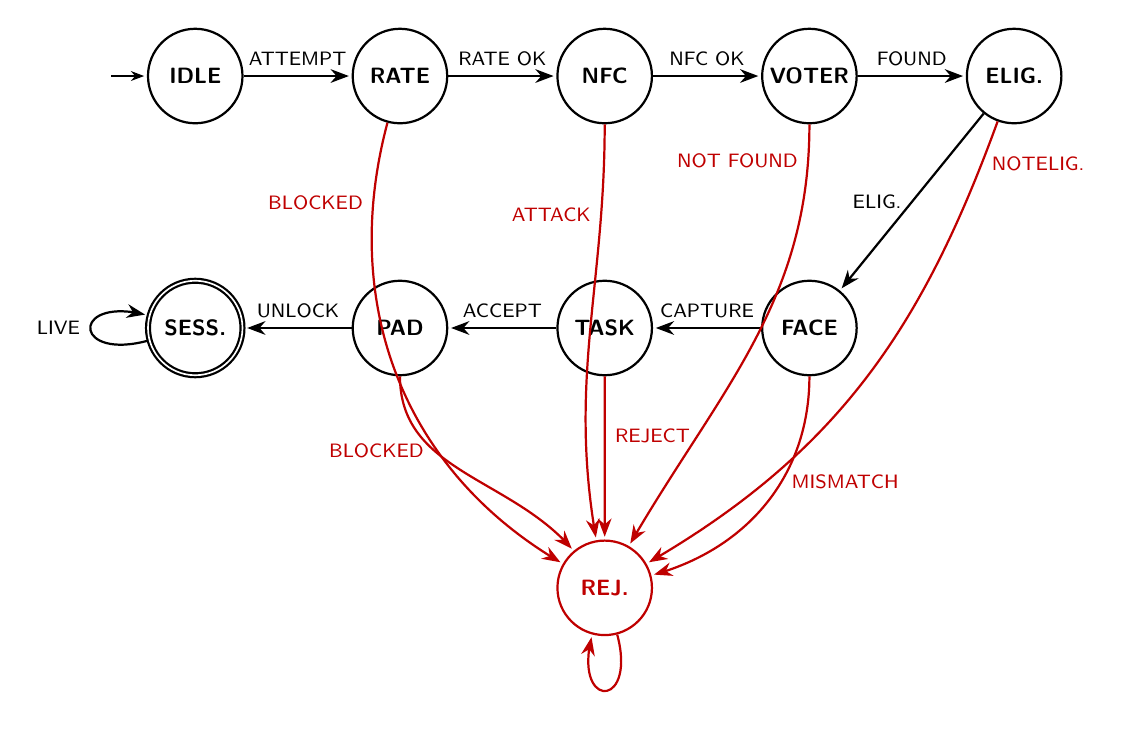
\begin{tikzpicture}[
  >=Stealth,
  shorten >=1pt,
  every state/.style={
    draw, circle, minimum size=1.2cm,
    font=\footnotesize\bfseries\sffamily, inner sep=1pt, thick
  },
  strans/.style={->, thick, font=\scriptsize\sffamily},
  ftrans/.style={->, thick, red!75!black,
                 font=\scriptsize\sffamily\color{red!75!black}}
]

%--- Explicit node placement ---
\node[state, initial, initial text={}] (idle)  at (0,   0)   {IDLE};
\node[state]                           (rate)  at (2.6, 0)   {RATE};
\node[state]                           (nfc)   at (5.2, 0)   {NFC};
\node[state]                           (voter) at (7.8, 0)   {VOTER};
\node[state]                           (elig)  at (10.4,0)   {ELIG.};

\node[state, accepting]                (sess)  at (0,  -3.2) {SESS.};
\node[state]                           (pad)   at (2.6,-3.2) {PAD};
\node[state]                           (task)  at (5.2,-3.2) {TASK};
\node[state]                           (face)  at (7.8,-3.2) {FACE};

\node[state, draw=red!75!black,
      text=red!75!black]               (rej)   at (5.2,-6.5) {REJ.};

%--- Success path ---
\path[strans]
  (idle)  edge node[above] {ATTEMPT} (rate)
  (rate)  edge node[above] {RATE OK} (nfc)
  (nfc)   edge node[above] {NFC OK}  (voter)
  (voter) edge node[above] {FOUND}   (elig)
  (elig)  edge node[left]  {ELIG.}   (face)
  (face)  edge node[above] {CAPTURE} (task)
  (task)  edge node[above] {ACCEPT}  (pad)
  (pad)   edge node[above] {UNLOCK}  (sess)
  (sess)  edge[loop left]  node[left] {LIVE} (sess);

%--- Failure transitions (out/in angles to avoid overlaps) ---
\path[ftrans]
  % RATE→REJ — exits bottom-left, label near source
  (rate)  edge[out=255, in=150]
          node[pos=0.15, left] {BLOCKED}   (rej)
  % NFC→REJ — exits straight down, label left of arc
  (nfc)   edge[out=270, in=100]
          node[pos=0.2, left]  {ATTACK}    (rej)
  % VOTER→REJ — label placed just below VOTER, to the left
  (voter) edge[out=270, in=60]
          node[pos=0.07, left] {NOT FOUND} (rej)
  % ELIG→REJ — label placed just below ELIG., to the right
  (elig)  edge[out=250, in=30]
          node[pos=0.07, right] {NOTELIG.} (rej)
  % FACE→REJ — exits bottom-right, label right midpoint
  (face)  edge[out=270, in=15]
          node[pos=0.4, right]  {MISMATCH} (rej)
  % TASK→REJ — exits straight down
  (task)  edge[out=270, in=90]
          node[pos=0.35, right] {REJECT}   (rej)
  % PAD→REJ — exits bottom, slight bend
  (pad)   edge[out=270, in=130]
          node[pos=0.35, left]  {BLOCKED}  (rej)
  % Trap self-loop
  (rej)   edge[loop below] node {} (rej);

\end{tikzpicture}
\end{document}
